\documentclass[a4paper,11pt]{book}
%\documentclass[a4paper,twoside,11pt,titlepage]{book}
\usepackage{listings}
\usepackage[utf8]{inputenc}
\usepackage[spanish]{babel}
\usepackage{float}

% \usepackage[style=list, number=none]{glossary} %
%\usepackage{titlesec}
%\usepackage{pailatino}

\decimalpoint
\usepackage{dcolumn}
\newcolumntype{.}{D{.}{\esperiod}{-1}}
\makeatletter
\addto\shorthandsspanish{\let\esperiod\es@period@code}
\makeatother


%\usepackage[chapter]{algorithm}
\RequirePackage{verbatim}
%\RequirePackage[Glenn]{fncychap}
\usepackage{fancyhdr}
\usepackage{graphicx}
\usepackage{afterpage}

\usepackage{longtable}

\usepackage[pdfborder={000}]{hyperref} %referencia

\usepackage[backend=biber, style=numeric, sorting=ynt]{biblatex}
\renewbibmacro{in:}{}

% \usepackage[
%     a4paper,
%     left=2.8cm,
%     right=2.7cm,
%     top=4cm,
%     bottom=3cm
% ]{geometry}

% ********************************************************************
% Re-usable information
% ********************************************************************
\newcommand{\myTitle}{Título del proyecto\xspace}
\newcommand{\myDegree}{Grado en ...\xspace}
\newcommand{\myName}{Nombre Apllido1 Apellido2 (alumno)\xspace}
\newcommand{\myProf}{Nombre Apllido1 Apellido2 (tutor1)\xspace}
\newcommand{\myOtherProf}{Nombre Apllido1 Apellido2 (tutor2)\xspace}
%\newcommand{\mySupervisor}{Put name here\xspace}
\newcommand{\myFaculty}{Escuela Técnica Superior de Ingenierías Informática y de
Telecomunicación\xspace}
\newcommand{\myFacultyShort}{E.T.S. de Ingenierías Informática y de
Telecomunicación\xspace}
\newcommand{\myDepartment}{Departamento de ...\xspace}
\newcommand{\myUni}{\protect{Universidad de Granada}\xspace}
\newcommand{\myLocation}{Granada\xspace}
\newcommand{\myTime}{\today\xspace}
\newcommand{\myVersion}{Version 0.1\xspace}


\hypersetup{
pdfauthor = {\myName (email (en) ugr (punto) es)},
pdftitle = {\myTitle},
pdfsubject = {},
pdfkeywords = {palabra_clave1, palabra_clave2, palabra_clave3, ...},
pdfcreator = {LaTeX con el paquete ....},
pdfproducer = {pdflatex}
}

%\hyphenation{}


%\usepackage{doxygen/doxygen}
%\usepackage{pdfpages}
\usepackage{url}
\usepackage{colortbl,longtable}
\usepackage[stable]{footmisc}
%\usepackage{index}

%\makeindex
%\usepackage[style=long, cols=2,border=plain,toc=true,number=none]{glossary}
% \makeglossary

% Definición de comandos que me son tiles:
%\renewcommand{\indexname}{Índice alfabético}
%\renewcommand{\glossaryname}{Glosario}

\pagestyle{fancy}
\fancyhf{}
\fancyhead[LO]{\leftmark}
\fancyhead[RE]{\rightmark}
\fancyhead[RO,LE]{\textbf{\thepage}}
\renewcommand{\chaptermark}[1]{\markboth{\textbf{#1}}{}}
\renewcommand{\sectionmark}[1]{\markright{\textbf{\thesection. #1}}}

\setlength{\headheight}{1.5\headheight}

\newcommand{\HRule}{\rule{\linewidth}{0.5mm}}
%Definimos los tipos teorema, ejemplo y definición podremos usar estos tipos
%simplemente poniendo \begin{teorema} \end{teorema} ...
\newtheorem{teorema}{Teorema}[chapter]
\newtheorem{ejemplo}{Ejemplo}[chapter]
\newtheorem{definicion}{Definición}[chapter]

\definecolor{gray97}{gray}{.97}
\definecolor{gray75}{gray}{.75}
\definecolor{gray45}{gray}{.45}
\definecolor{gray30}{gray}{.94}

\lstset{ frame=Ltb,
     framerule=0.5pt,
     aboveskip=0.5cm,
     framextopmargin=3pt,
     framexbottommargin=3pt,
     framexleftmargin=0.1cm,
     framesep=0pt,
     rulesep=.4pt,
     backgroundcolor=\color{gray97},
     rulesepcolor=\color{black},
     %
     stringstyle=\ttfamily,
     showstringspaces = false,
     basicstyle=\scriptsize\ttfamily,
     commentstyle=\color{gray45},
     keywordstyle=\bfseries,
     %
     numbers=left,
     numbersep=6pt,
     numberstyle=\tiny,
     numberfirstline = false,
     breaklines=true,
   }
 
% minimizar fragmentado de listados
\lstnewenvironment{listing}[1][]
   {\lstset{#1}\pagebreak[0]}{\pagebreak[0]}

\lstdefinestyle{CodigoC}
   {
	basicstyle=\scriptsize,
	frame=single,
	language=C,
	numbers=left
   }
\lstdefinestyle{CodigoC++}
   {
	basicstyle=\small,
	frame=single,
	backgroundcolor=\color{gray30},
	language=C++,
	numbers=left
   }

 
\lstdefinestyle{Consola}
   {basicstyle=\scriptsize\bf\ttfamily,
    backgroundcolor=\color{gray30},
    frame=single,
    numbers=none
   }


\newcommand{\bigrule}{\titlerule[0.5mm]}


%Para conseguir que en las páginas en blanco no ponga cabecerass
\makeatletter
\def\clearpage{%
  \ifvmode
    \ifnum \@dbltopnum =\m@ne
      \ifdim \pagetotal <\topskip
        \hbox{}
      \fi
    \fi
  \fi
  \newpage
  \thispagestyle{empty}
  \write\m@ne{}
  \vbox{}
  \penalty -\@Mi
}
\makeatother

\usepackage{pdfpages}


\addbibresource{bibliografia/bibliografia.bib}
\addbibresource{bibliografia/webs.bib}

\begin{document}
\begin{titlepage}
 
 
\newlength{\centeroffset}
\setlength{\centeroffset}{-0.5\oddsidemargin}
\addtolength{\centeroffset}{0.5\evensidemargin}
\thispagestyle{empty}

\noindent\hspace*{\centeroffset}\begin{minipage}{\textwidth}

\centering

\includegraphics[width=0.9\textwidth]{imagenes/logo_ugr.jpg}\\[1.4cm]

\textsc{ \Large TRABAJO FIN DE GRADO\\[0.2cm]}
\textsc{ INGENIERÍA EN ...}\\[1cm]
% Upper part of the page
% 
% Title
{\Huge\bfseries Titulo del Proyecto\\
}
\noindent\rule[-1ex]{\textwidth}{3pt}\\[3.5ex]
{\large\bfseries Subtitulo del Proyecto}
\end{minipage}

\vspace{2.5cm}
\noindent\hspace*{\centeroffset}\begin{minipage}{\textwidth}
\centering

\textbf{Autor}\\ {Nombre Apellido1 Apellido2 (alumno)}\\[2.5ex]
\textbf{Directores}\\
{Nombre Apellido1 Apellido2 (tutor1)\\
Nombre Apellido1 Apellido2 (tutor2)}\\[2cm]

\includegraphics[width=0.3\textwidth]{imagenes/etsiit_logo.png}\\[0.1cm]
\textsc{Escuela Técnica Superior de Ingenierías Informática y de Telecomunicación}\\
\textsc{---}\\
Granada, mes de 201
\end{minipage}
%\addtolength{\textwidth}{\centeroffset}
%\vspace{\stretch{2}}
\end{titlepage}



\chapter*{}
%\thispagestyle{empty}
%\cleardoublepage

%\thispagestyle{empty}

\thispagestyle{empty}

\begin{center}
{\large\bfseries Etiquetado de imágenes en química}\\
\end{center}
\begin{center}
Pedro Bedmar López\\
\end{center}

%\vspace{0.7cm}
\noindent{\textbf{Palabras clave}: palabra\_clave1, palabra\_clave2, palabra\_clave3, ......}\\

\vspace{0.7cm}
\noindent{\textbf{Resumen}}\\

Poner aquí el resumen.
\cleardoublepage


\thispagestyle{empty}


\begin{center}
{\large\bfseries Image labelling in chemistry}\\
\end{center}
\begin{center}
Pedro Bedmar López\\
\end{center}

%\vspace{0.7cm}
\noindent{\textbf{Keywords}: Keyword1, Keyword2, Keyword3, ....}\\

\vspace{0.7cm}
\noindent{\textbf{Abstract}}\\

Write here the abstract in English.



\begin{flushright}
Granada a X de mes de 201 .
\end{flushright}


\chapter*{}
\thispagestyle{empty}

\noindent\rule[-1ex]{\textwidth}{2pt}\\[4.5ex]

Dña. \textbf{Rocío Celeste Romero Zaliz}, Profesora Titular del Departamento de Ciencias de la Computación e Inteligencia Artificial de la Universidad de Granada.


\vspace{0.5cm}

\textbf{Informa:}

\vspace{0.5cm}

Que el presente trabajo, titulado \textit{\textbf{Etiquetado de imágenes en química}},
ha sido realizado bajo su supervisión por \textbf{Pedro Bedmar López}, y autoriza la defensa de dicho trabajo ante el tribunal que corresponda.

\vspace{0.5cm}

Y para que conste, expide y firma el presente informe en Granada a X de julio de 2022.

\vspace{1cm}

\textbf{La directora:}

\vspace{5cm}

\noindent \textbf{Rocío Celeste Romero Zaliz}

\chapter*{Agradecimientos}
\thispagestyle{empty}

       \vspace{1cm}


Poner aquí agradecimientos...


\frontmatter
\tableofcontents
\listoffigures
\listoftables

\mainmatter
\setlength{\parskip}{5pt}

\chapter{Introducción}

Debido al desarrollo exponencial de la informática en el último siglo, todas las ramas del conocimiento se han visto afectadas. La informática está permitiendo la automatización de muchas tareas que anteriormente se realizaban de forma manual por un operario. 

Con el paso de los años, esta capacidad de automatización va en aumento pudiéndose aplicar en situaciones anteriormente impensables. Los numerosos avances en hardware y la aplicación de arquitecturas GPU en el campo del Aprendizaje Automático, y concretamente del Deep Learning, han permitido crear modelos mucho más avanzados capaces de interiorizar datos más complejos. 

La química es una de las ciencias que se ha impregnado de este desarrollo tecnológico y de esta combinación ha surgido lo que se conoce como cheminformatics o chemoinformatics. En este capítulo definiremos esta rama científica y describiremos sus principales actuaciones. A continuación, explicaremos distintos conceptos y tecnologías existentes relacionados con el proyecto.

\section{Motivación del proyecto}
Desde hace décadas, en el mundo de la química ha estado presente la necesidad de almacenar, gestionar y procesar la gran cantidad de información que se genera. Con el tiempo se fueron desarrollando técnicas de tratamiento de ésta, pero no fue hasta hace algunos años cuando se acuñó el nombre de cheminformatics o chemoinformatics. 

En la literatura existen diferentes definiciones para este término, discutidas en \cite{doi:10.1021/ci600234z}. \\
``Chem(o)informatics es un término genérico que encompasa el diseño, creación, gestión, recuperación, análisis, diseminación, visualización y el uso de información química'' es una de las definiciones recogidas. Otra más abierta es ``La aplicación de métodos informáticos para resolver problemas de química''. 

% TODO: para qué necesitan los científicos de Negev un clasificador de imágenes?
Desde la Universidad de Granada, mi tutora Rocío trabaja en este ámbito. Colabora con químicos de la Universidad de Negev y es consciente de los problemas que tienen para manejar la gran cantidad de datos que aparecen en publicaciones científicas. Un tipo de datos muy valioso son las imágenes, pero clasificarlas no es trivial: pueden ser sobre cualquier temática, algunas pueden referirse a esquemas explicando cómo funciona un modelo, otras pueden contener resultados de algún experimento, pueden ser representaciones de compuestos químicos, etc. Clasificarlas manualmente por un operario no es una opción viable.

Otra necesidad que tienen estos científicos es la de conseguir más imágenes: etiquetarlas de forma manual es una tarea tediosa.

Es por ello que en este Trabajo de Fin de Grado vamos a crear dos utilidades, un generador de imágenes sintéticas (tanto de imágenes de moléculas como de ejemplos negativos) y un modelo que permita clasificar imágenes. En concreto, aquellas que son representaciones de moléculas organometálicas, del resto.

Aunque existen diferentes opiniones sobre el alcance de las cheminformatics, se puede considerar que este proyecto está dentro de sus fronteras, ya que vamos a crear una herramienta de clasificación de imágenes químicas, es decir, una herramienta que procesa y analiza este tipo de información.

\chapter*{Planificación del proyecto}
En los primeros años del desarrollo de software, este se creaba sin seguir ningun enfoque formal. Muchos de los proyectos que se iniciaban terminaban fracasando por los retrasos en la entrega, el mal funcionamiento del producto o por no cumplir los requisitos del cliente. Además, la complejidad requerida en el software iba aumentando con el tiempo. 

Por ello, era necesario crear un marco que permitiera metodizar el desarrollo. Es así como surge la Ingeniería del Software, que acompaña al software durante todo su ciclo vital.

En nuestro proyecto vamos a aplicar este enfoque a la hora de desarrollar el producto, y en este apartado vamos a describir información general sobre su gestión, la metodología de desarrollo a seguir y otra información relativa a costes, riesgos y otros factores que influyen sobre el proyecto para asegurarnos de que se consiguen los objetivos en el tiempo previsto, detectando posibles amenazas y problemas a tiempo.

\section*{Gestión del proyecto}

\section*{Metodología de desarrollo}

Las metodologías se pueden clasificar en dos grandes bloques \cite{metodologiasDesarrollo}, tradicionales y ágiles. Las tradicionales son las que primero surgieron, se caracterizan por definir rígidamente los requisitos al inicio del proyecto. En ellas, se aplica una serie de etapas de forma lineal, y una vez alcanzada una de ellas no se puede volver atrás. Por todo esto no se adaptan bien a los cambios.

En general, los proyectos de software tienden a ser cada vez más complejos. Las metodologías ágiles surgieron con el objetivo de hacer los proyectos de desarrollo más dinámicos, de forma que se adaptaran mejor al entorno y a los cambios. Se basan en una metodología incremental, donde se van construyendo prototipos del producto poco a poco, añadiendo funcionalidades hasta obtener la aplicación final. Los equipos se reunen cada poco tiempo para intercambiar ideas y repartir las tareas a realizar.

A la hora de elegir la metodología que vamos a usar, debemos tener en cuenta los siguientes factores relativos a la naturaleza del proyecto:

\begin{itemize}
    \item Se trata de un proyecto de investigación, donde vamos a aplicar diferentes técnicas de Aprendizaje Automático a la resolución de un problema. Por tanto, a priori no se conoce la calidad de los resultados que se van a obtener y el número y tipo de experimentos que va a ser necesario realizar.
    \item La intervención del experto en química va a ser fundamental durante el desarrollo del proyecto. Aportará información y feedback esencial durante todas las fases.
\end{itemize}

Por estas razones, creemos que la metodología de desarrollo que mejor se adapta a nuestras necesidades es una metodología ágil, ya que nos provee de gran flexibilidad, permitiendo el desarrollo del proyecto de una forma incremental donde obtenemos feedback del cliente y del experto en cada iteración.

Revisando las distintas metodologías \cite{despa2014comparative}, creemos que una buena candidata es SCRUM \cite{schwaber1997scrum}. Es posiblemente una de las más utilizadas en la actualidad, y los proyectos que la aplican cuentan con las siguientes características:

\begin{itemize}
    \item \textbf{Entregable flexible:} Su contenido viene dado por lo que demanda el entorno. 
    \item \textbf{Calendario flexible:} El entregable puede ser requerido antes o después de lo previsto.
    \item \textbf{Equipos pequeños:} Los equipos están formados por pocas personas, de forma que la comunicación y sincronización entre sus miembros es alta. 
    \item \textbf{Revisiones frecuentes:} El progreso del equipo se evalúa de forma periódica y frecuentemente, de forma que se ponen en común las dificultades encontradas y se intentan resolver con la ayuda de todos los miembros.
    \item \textbf{Colaboración:} La colaboración entre todos los miembros del equipo es muy alta, así como entre el equipo y entidades externas como el cliente.
\end{itemize}

Cuando se trabaja con esta metodología, en cada equipo existe un miembro conocido como SCRUM manager. Es el encargado de guiar al equipo en el desarrollo y en la aplicación de la metodología. En SCRUM el equipo es muy importante y todos sus miembros participan con su opinión. Esta metodología consta de las siguientes fases:

% TODO: Si fuera necesario, añadir información sobre los tipos de equipos. En el paper de SCRUM aparece información sobre estos.

\begin{figure}[H]
    \centering
        \fbox{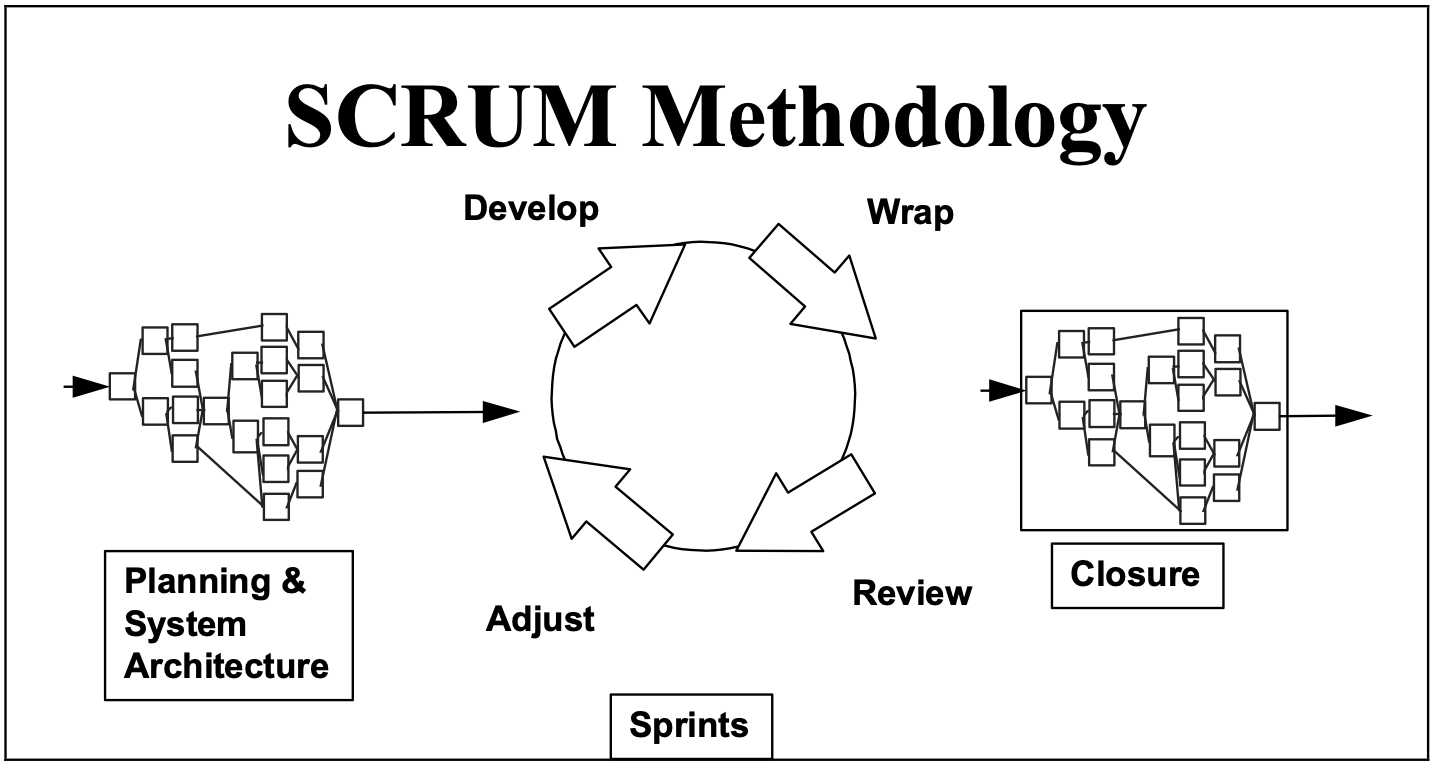
\includegraphics[scale=0.45]{imagenes/scrum.png}}  
        \caption{Fases de la metodología SCRUM \cite{schwaber1997scrum}} \label{fig:figura1}
    \end{figure}

\begin{itemize}
    \item \textbf{Pregame:} 
    \begin{itemize}
        \item \textit{Planificación:} En esta fase se crea la lista de tareas a realizar (backlog list), se fija la fecha de entrega del producto y su funcionalidad, se forma el equipo (o equipos) de trabajo, se valoran los riesgos que puedan surgir, los costes y finalmente se revisa todo y se aprueba el proyecto.
        \item \textit{Arquitectura/Diseño de alto nivel:} Se revisan los elementos en el backlog, se realizan cambios si es necesario para poder implementarlos, se perfila la arquitectura del sistema teniendo en cuenta estos cambios y una reunión es organizada para revisar el diseño, donde cada equipo presenta una propuesta para implementar cada backlog.
    \end{itemize}
    \item \textbf{Game:} Corresponde con el conocido Sprint de la metodología SCRUM. Es la parte iterativa de la metodología, que se ejecuta varias veces hasta conseguir el producto final y está formada por las siguientes subtareas:
    \begin{itemize}
        \item \textit{Desarrollo:} Lo primero que se realiza es definir los cambios que hay que realizar en los backlogs para poder implementarlos. Se dividen las tareas presentes en el backlog en paquetes, y se completan estos paquetes diseñando, desarrollando, implementando, testeando y documentando los cambios.
        \item \textit{Envoltura:} Se cierran los paquetes, creando una ejecutable que incorpora los cambios y se explica como cumplen lo especificado en los backlogs.
        \item \textit{Revisión:} Todos los equipos se reunen para presentar el trabajo. El desarrollo obtenido se evalúa y se añaden nuevas tareas que puedan surgir al backlog. Se evalúa el riesgo y se realizan propuestas en base a este.
        \item \textit{Ajuste:} Se consolida la información recibida durante la revisión.
    \end{itemize}
    
    \item \textbf{Postgame:}
    \begin{itemize}
        \item \textit{Cierre:} Cuando el gestor del proyecto considera que el producto está terminado y cumple con los requisitos solicitados por el cliente se entra en esta fase, donde se prepara el producto para su despliegue. Integración, generación de la documentación, testeo y marketing son algunas de las actividades que se realizan en este paso.
    \end{itemize}

\end{itemize}

Estas características que hemos mencionado son las especificadas en la definición original de SCRUM. Aún así, en la práctica cada proyecto las adapta a sus necesidades. En general, los sprints suelen tener una duración de 2 o 3 semanas. En nuestro caso tendrán 1 o 2 semanas de duración.



\chapter*{Estado del arte}
Para poder organizar este proyecto, debemos conocer el estado del arte en su ámbito. Como comentamos en la introducción, cheminformatics es un tema muy amplio y engloba subtópicos diferentes. Muchos de ellos surgieron en la década de 1960 y principios de 1970, y desde esa época muchos grupos de investigación siguen trabajando en ellos y nuevos grupos han surgido para aplicar nuevas tecnologías en nuevos ámbitos. A continuación discutimos algunos de los temas que históricamente han sido de interés para esta ciencia. \cite{doi:10.1021/ci600234z}

\section*{Compuestos orgánicos y su representación}
Un compuesto orgánico es un compuesto químico que contiene átomos de carbono, formando enlaces carbono-carbono y carbono-hidrógeno \cite{comporganico}. En este TFG, vamos a trabajar concretamente con la clasificación de compuestos organometálicos, donde los átomos de carbono forman enlaces covalentes con átomos metálicos \cite{comporganometalico}.

En las publicaciones de química encontramos numerosas representaciones gráficas de estos compuestos, lo que se conocen como fórmulas estructurales. Éstas muestran la disposición en el espacio de los átomos que forman el compuesto. Un ejemplo es la siguiente figura:

\begin{figure}[H]
\centering
    \fbox{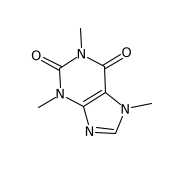
\includegraphics[scale=0.7]{imagenes/caffeine.png}}  
    \caption{Estructura de la cafeína} \label{fig:figura1}
\end{figure}

\noindent En ellas pueden aparecer multitud de elementos, apareciendo siempre:
\begin{itemize}
    \item \textbf{Átomos:} Se sitúan en los extremos de los enlaces. Representados con letras que indican el elemento químico del que se trata, tal y como aparece en la tabla periódica.
    \item \textbf{Enlaces:} Unen dos átomos entre sí. 
\end{itemize}

 En algunas ocasiones, sobre los átomos pueden mostrarse cargas positivas o negativas representando iones. Aparte, puede mostrarse lo que se conoce como información estereoquímica, que indica la disposición de los átomos en el espacio. Ésta es importante ya que afecta a las propiedades y reactividad de las moléculas \cite{estereoquimica,structrep}.

 \begin{figure}[H]
\centering
    \fbox{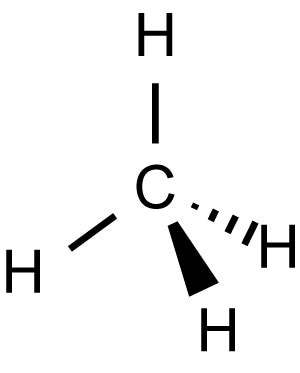
\includegraphics[scale=0.5]{imagenes/methane.jpg}}  
    \caption{Estructura del metano} \label{fig:figura2}
\end{figure}

\begin{itemize}
    \item Las líneas sólidas representan enlaces en el plano.
    \item Las discontinuas representan enlaces que están más alejados.
    \item Aquellas con forma de cuña indican que uno de los átomos se encuentra más cerca del espectador. 
\end{itemize}

Además, un mismo compuesto se puede representar de distintas formas:
\begin{figure}[H]
\centering
    \fbox{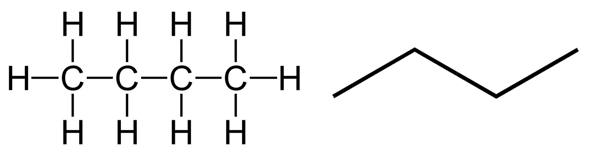
\includegraphics[scale=0.5]{imagenes/skeletal.png}}  
    \caption{Dos formas de representar el butano} \label{fig:figura2}
\end{figure}

A la izquierda se detalla la definición de todos los átomos, en cambio a la derecha encontramos lo que se conoce como fórmula de esqueleto, donde se omiten los átomos de carbono e hidrógeno. Se sabe que hay un átomo de carbono en los vértices que quedan libres en la intersección de dos enlaces o en las terminaciones donde no aparece ningún otro elemento. Se supone a la vez que cada átomo de carbono tiene cuatro enlaces, por tanto el número de enlaces que faltan por indicar explícitamente se corresponden con enlaces a moléculas de hidrógeno \cite{formestructural,structrep}.


\section*{Representación en el ordenador}
El poder almacenar representaciones de compuestos químicos de manera eficiente en un ordenador requiere de la creación de métodos y formatos específicos para ello. Además, hay que tener en cuenta qué datos vamos a codificar, si solo la estructura básica del compuesto, si también queremos guardar información estereoquímica o si queremos añadir notas auxiliares sobre los compuestos. Es importante tener esto claro, ya que la complejidad de la representación influirá en la cantidad de almacenamiento que ocupe en disco y en los recursos necesarios para procesarla.

Utilizando notación lineal, representamos la estructura del compuesto como una secuencia lineal de caracteres y números. Esta es una codificación adecuada para las computadoras, ya que la pueden procesar con facilidad. Algunos formatos que utilizan esta notación son WLN (Wiswesser Line Notation), ROSDAL (Rp) o SMILES (Simplified Molecular Input Line Entry Specification). Aunque WLN y ROSDAL han quedado obsoletos, SMILES se sigue utilizando con mucha frecuencia en la actualidad. \cite{doi:10.1021/ci600234z}

\begin{figure}[H]
\centering
    \fbox{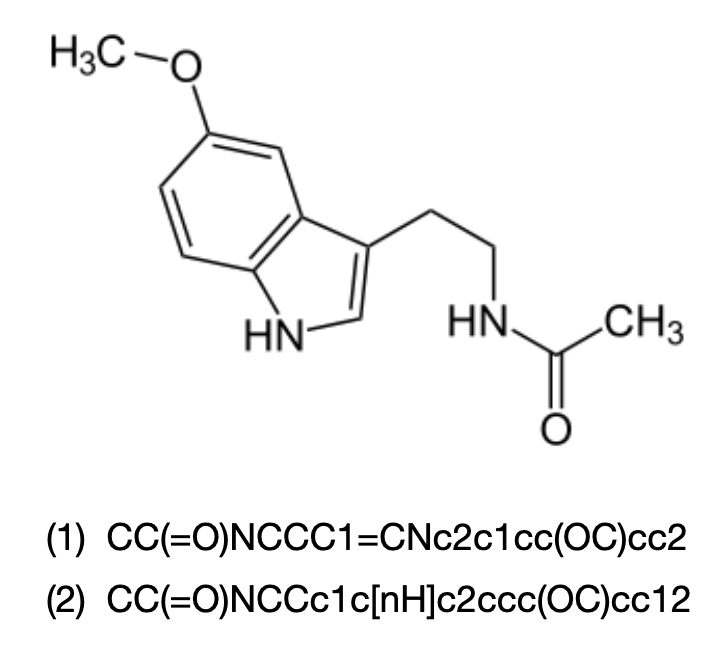
\includegraphics[scale=0.25]{imagenes/smiles_melatonina.png}}  
    \caption{Dos posibles codificaciones de la melatonina en SMILES \cite{smiles_wikipedia}} \label{fig:figura2}
\end{figure}

Aunque no vamos a entrar en detalle de cómo funciona, ya que para ello hay que tener nociones avanzadas de química, diremos que utiliza las siglas de cada elemento de la tabla periódica para representar los átomos. La primera letra del elemento se escribe en mayúscula, a no ser que se trate de un átomo perteneciente a un anillo aromático\footnote{La aromaticidad es una propiedad presente en enlaces dobles de moléculas cíclicas, donde sus electrones pueden circular libremente. Esto mejora la estabilidad del compuesto. \cite{aromaticidad, aromaticidad_wikipedia}}, ya que en ese caso se escribe en minúscula. Si el elemento tiene dos caracteres, el segundo se escribe siempre en minúscula. Además, se pueden representar cargas.

Los enlaces se representan con -, =, \# y :, según el tipo. Bajo algunas circunstancias, se pueden omitir estos símbolos, ya que por su contexto se deducen. También se pueden codificar ramas, situando elementos entre paréntesis, y ciclos, utilizando un número para indicar el inicio y el fin del ciclo en la cadena de texto. \cite{weininger1988smiles}

\begin{figure}[H]
\centering
    \fbox{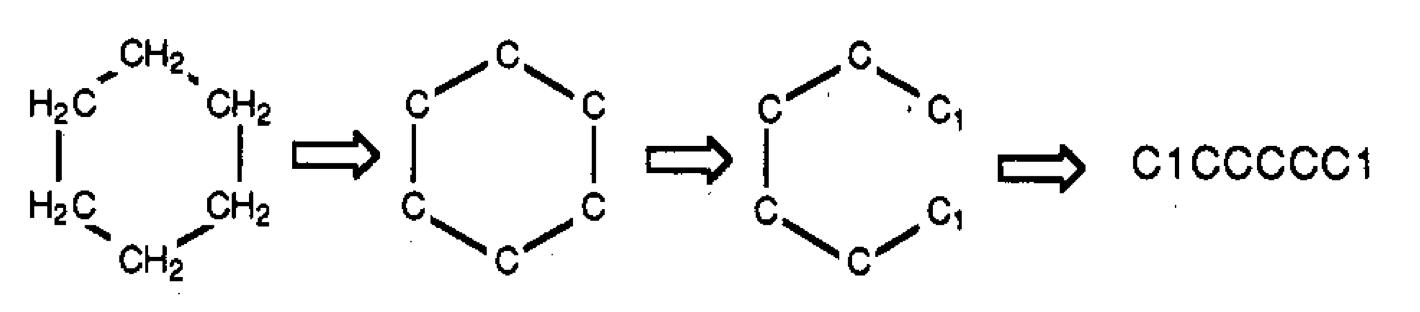
\includegraphics[scale=0.35]{imagenes/smiles_cycle.png}}  
    \caption{Ciclos en SMILES} \label{fig:figura2}
\end{figure}

Otras características como la aromaticidad o estructuras inconectas también pueden ser representadas. Entre las ventajas de esta codificación, destaca su facilidad de comprensión por los humanos. Cualquier químico puede aprender sus reglas de codificación fácilmente y diseñar sus propios compuestos. Un problema que tiene SMILES es que un mismo elemento se puede representar de diferentes formas. Pero sobre todo, el mayor problema es que un porcentaje significativo de las cadenas no se corresponden con moléculas válidas, ya sea porque son sintácticamente inválidas, no se corresponden con un grafo molecular o no cumplen reglas químicas básicas. \cite{weininger1988smiles}

Uno de los principales objetivos de la química computacional es el diseño de nuevas moléculas. Para ello, la utilización de modelos generativos puede ayudar a los investigadores, pero si el espacio de estados de SMILES no es completamente válido se dificulta la tarea. Para ello han surgido otras codificaciones como SELFIES con un espacio 100\% robusto. \cite{Krenn_2020}

Además de estos formatos de notación lineal, es necesario mencionar otros. El lanzamiento en 1982 de MDL Molfile llevó a su aceptación como principal formato para representar datasets químicos. Se han realizado distintas adaptaciones de este para añadir información extra a las moléculas, dando lugar a SDfile, RGfile, Rxnfile, etc. El formato PDB se utiliza principalmente para almacenar información 3D de macromoléculas biológicas, como son las proteínas o los polinucleótidos. CIF también es un formato para almacenar información 3D. En espectroscopia encontramos JCAMP. Finalmente, CML (chemical markup language), una extensión de XML, es una propuesta que intenta aglutinar toda la información disponible. Es compatible con moléculas, reacciones, espectroscopia y otra información. \cite{doi:10.1021/ci600234z}

\begin{figure}[H]
\centering
    \fbox{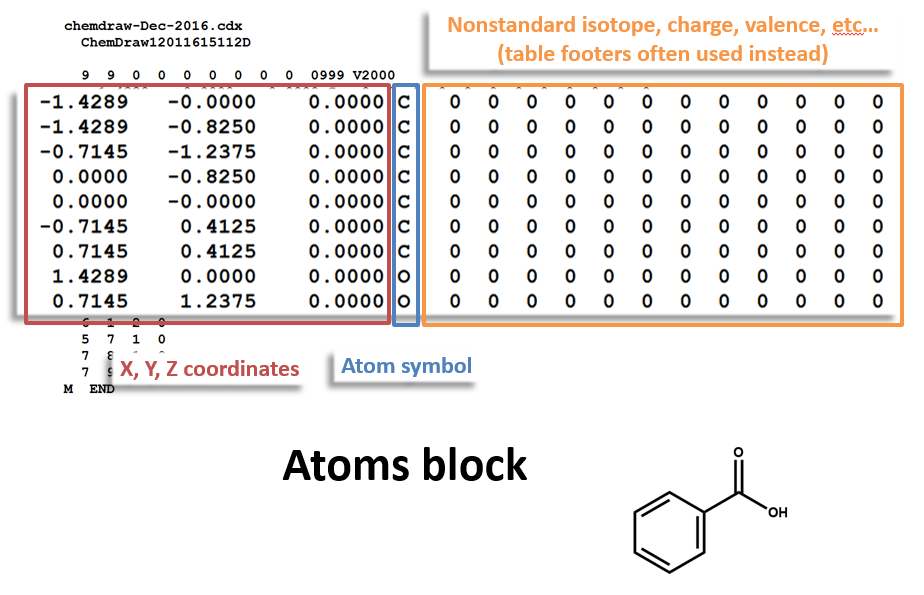
\includegraphics[scale=0.3]{imagenes/molfile.png}}  
    \caption{Contenido de un archivo MOL \cite{molfile_example}} \label{fig:figura2}
\end{figure}


\section*{Fuentes y bases de datos}

El gran número de facetas que presenta la información química necesita sistemas de almacenamiento a la altura. La química fue una de las primeras ramas científicas en utilizar bases de datos para almacenar: la cantidad de datos que se generaba creció rápidamente, y sigue creciendo hoy en día. 

Aunque es muy complicado clasificarlas, vamos a separarlas en tres grandes grupos según el tipo de información que almacenan: \cite{doi:10.1021/ci600234z}
\begin{itemize}
    \item \textbf{Bases de datos de publicaciones:} Pueden ser bibliográficas, guardando solamente los metadatos y la referencia a la publicación, o de texto completo, donde recogen la publicación de forma íntegra. %TODO: Qué son las publicaciones primarias?
    \item \textbf{Bases de datos fácticas:} Al contrario que las anteriores, que almacenan publicaciones de la literatura primaria, estas pueden guardar propiedades físicas de compuestos, información de espectroscopia, información legal, etc.
    \item \textbf{Bases de datos de estructuras y reacciones:} Recogen estructuras químicas, tanto individualmente como formando parte de reacciones. No se almacenan como imágenes, sino en formatos interpretables por la máquina.
    \item \textbf{Bases de datos de biología molecular:} Contienen secuencias de aminoácidos y nucleótidos.
\end{itemize}

Pero, ¿cómo podemos rellenarlas con datos? ¿De dónde podemos extraerlos? Durante décadas se han publicado un gran número de artículos. Podríamos utilizarlos como una fuente muy amplia de información, ya que contienen todo el progreso científico. Específicamente para extraer datos relativos a estructuras, entran en juego utilidades conocidas como OCSR (Optical Chemical Structure Recognition).

Son capaces de transformar una imagen en un formato compatible con la máquina, como podría ser SMILES. En muchos casos incluso es posible introducirles una publicación completa y ellas mismas localizan las imágenes de moléculas. Con el paso del tiempo se han ido perfeccionando, y algunas son capaces de detectar información estereoquímica o de relacionar el compuesto con el texto de la publicación. Más adelante repasaremos algunas de estas utilidades. 

Por último, mencionar una base de datos que merece la pena conocer. Creada por el National Institute of Health (NIH), PubChem es una base de datos abierta que cada mes sirve a millones de usuarios en todo el mundo. Es una base de datos de estructuras y aunque contiene mayoritariamente moléculas pequeñas, también almacena nucleótidos, carbohidratos, lípidos, péptidos y macromoléculas modificadas químicamente. Para cada compuesto almacena su estructura, identificadores, propiedades físicas y químicas, toxicidad, patentes, etc. Los datos que aglutina provienen de diversas fuentes, como son agencias del gobierno estadounidense, editores de revistas científicas o proveedores químicos, aunque hay muchas más. \cite{pubchem}

\section*{Métodos de búsqueda}
Almacenar información en las bases de datos no sirve de nada si no se desarrollan métodos eficientes para extraerla. En aquellas bases de datos donde se almacenan estructuras químicas, una de las principales formas de obtener información es buscar similitudes entre una molécula dada como entrada y otras que se encuentran almacenadas, de forma que compartan una subestructura específica o tengan otras características en común. Para ello, es clave la codificación de los compuestos.

También, si se almacenan metadatos y la base de datos está indexada sobre ellos se podría buscar por su nombre, etiquetas, etc. \cite{doi:10.1021/ci600234z}


\section*{Métodos para análisis de datos}
En química, grandes cantidades de datos son producidas. Una vez que hemos conseguido limpiarlos y ordenarlos, tenemos un conocimiento muy valioso en nuestras manos. La información es muy interesante en sí misma, pero también lo son las relaciones que se esconden en su interior. Para ello, se crean modelos que puedan interiorizarlas.

El análisis de datos no solo se enfrenta a la extracción de la información principal, sino que también intenta generar nueva información secundaria. \cite{doi:10.1021/ci600234z}

Este TFG se desarrolla dentro de este ámbito, ya que, como describiremos más adelante, entrenamos un modelo capaz de detectar que imágenes contienen moléculas organometálicas. Además, creamos un modelo generativo para aumentar el tamaño del dataset en uso.
%
%\input{capitulos/02_EspecificacionRequisitos}
%
%\input{capitulos/04_Analisis}
%
%\input{capitulos/05_Diseno}
%
%\input{capitulos/06_Implementacion}
%
%\input{capitulos/07_Pruebas}
%
%\input{capitulos/08_Conclusiones}

%%\chapter{Conclusiones y Trabajos Futuros}
%
%

\printbibliography[nottype=online, title={Bibliografía}]
\printbibliography[type=online, title={Otras fuentes}]

% \printbibheading
% \printbibliography{nottype=misc, heading=subbibliography, title={Citas}}
% \printbibliography{type=misc, heading=subbibliography, title={Otras fuentes}}

% \nocite{*}
% \bibliography{bibliografia/bibliografia}{}
% \bibliographystyle{ieeetr}
% \addcontentsline{toc}{chapter}{Bibliografía}
% \bibliographystyle{miunsrturl}
%
%\appendix
%\input{apendices/manual_usuario/manual_usuario}
%%\input{apendices/paper/paper}
%\input{glosario/entradas_glosario}
% \addcontentsline{toc}{chapter}{Glosario}
% \printglossary
%\chapter*{}
\thispagestyle{empty}

\end{document}
